% Template for PLoS
% Version 3.5 March 2018
%
% % % % % % % % % % % % % % % % % % % % % %
%
% -- IMPORTANT NOTE
%
% This template contains comments intended 
% to minimize problems and delays during our production 
% process. Please follow the template instructions
% whenever possible.
%
% % % % % % % % % % % % % % % % % % % % % % % 
%
% Once your paper is accepted for publication, 
% PLEASE REMOVE ALL TRACKED CHANGES in this file 
% and leave only the final text of your manuscript. 
% PLOS recommends the use of latexdiff to track changes during review, as this will help to maintain a clean tex file.
% Visit https://www.ctan.org/pkg/latexdiff?lang=en for info or contact us at latex@plos.org.
%
%
% There are no restrictions on package use within the LaTeX files except that 
% no packages listed in the template may be deleted.
%
% Please do not include colors or graphics in the text.
%
% The manuscript LaTeX source should be contained within a single file (do not use \input, \externaldocument, or similar commands).
%
% % % % % % % % % % % % % % % % % % % % % % %
%
% -- FIGURES AND TABLES
%
% Please include tables/figure captions directly after the paragraph where they are first cited in the text.
%
% DO NOT INCLUDE GRAPHICS IN YOUR MANUSCRIPT
% - Figures should be uploaded separately from your manuscript file. 
% - Figures generated using LaTeX should be extracted and removed from the PDF before submission. 
% - Figures containing multiple panels/subfigures must be combined into one image file before submission.
% For figure citations, please use "Fig" instead of "Figure".
% See http://journals.plos.org/plosone/s/figures for PLOS figure guidelines.
%
% Tables should be cell-based and may not contain:
% - spacing/line breaks within cells to alter layout or alignment
% - do not nest tabular environments (no tabular environments within tabular environments)
% - no graphics or colored text (cell background color/shading OK)
% See http://journals.plos.org/plosone/s/tables for table guidelines.
%
% For tables that exceed the width of the text column, use the adjustwidth environment as illustrated in the example table in text below.
%
% % % % % % % % % % % % % % % % % % % % % % % %
%
% -- EQUATIONS, MATH SYMBOLS, SUBSCRIPTS, AND SUPERSCRIPTS
%
% IMPORTANT
% Below are a few tips to help format your equations and other special characters according to our specifications. For more tips to help reduce the possibility of formatting errors during conversion, please see our LaTeX guidelines at http://journals.plos.org/plosone/s/latex
%
% For inline equations, please be sure to include all portions of an equation in the math environment.  For example, x$^2$ is incorrect; this should be formatted as $x^2$ (or $\mathrm{x}^2$ if the romanized font is desired).
%
% Do not include text that is not math in the math environment. For example, CO2 should be written as CO\textsubscript{2} instead of CO$_2$.
%
% Please add line breaks to long display equations when possible in order to fit size of the column. 
%
% For inline equations, please do not include punctuation (commas, etc) within the math environment unless this is part of the equation.
%
% When adding superscript or subscripts outside of brackets/braces, please group using {}.  For example, change "[U(D,E,\gamma)]^2" to "{[U(D,E,\gamma)]}^2". 
%
% Do not use \cal for caligraphic font.  Instead, use \mathcal{}
%
% % % % % % % % % % % % % % % % % % % % % % % % 
%
% Please contact latex@plos.org with any questions.
%
% % % % % % % % % % % % % % % % % % % % % % % %

\documentclass[10pt,letterpaper]{article}
\usepackage[top=0.85in,left=2.75in,footskip=0.75in]{geometry}

% amsmath and amssymb packages, useful for mathematical formulas and symbols
\usepackage{amsmath,amssymb}

% Use adjustwidth environment to exceed column width (see example table in text)
\usepackage{changepage}

% Use Unicode characters when possible
% Codificação de entrada compatível com ambos os motores:
% pdfLaTeX carrega inputenc[utf8]; XeLaTeX/LuaLaTeX tratam UTF-8 nativamente.
\usepackage{iftex}
\ifPDFTeX
  \usepackage[utf8]{inputenc}
  \usepackage[T1]{fontenc}
\fi

% textcomp package and marvosym package for additional characters
\usepackage{textcomp,marvosym}

% cite package, to clean up citations in the main text. Do not remove.
\usepackage{cite}

% Use nameref to cite supporting information files (see Supporting Information section for more info)
\usepackage{nameref,hyperref}

% line numbers
\usepackage[right]{lineno}

% ligatures disabled
\usepackage{microtype}
\ifPDFTeX\DisableLigatures[f]{encoding = *, family = * }\fi

% color can be used to apply background shading to table cells only
\usepackage[table]{xcolor}

% array package and thick rules for tables
\usepackage{array}

% create "+" rule type for thick vertical lines
\newcolumntype{+}{!{\vrule width 2pt}}

% create \thickcline for thick horizontal lines of variable length
\newlength\savedwidth
\newcommand\thickcline[1]{%
  \noalign{\global\savedwidth\arrayrulewidth\global\arrayrulewidth 2pt}%
  \cline{#1}%
  \noalign{\vskip\arrayrulewidth}%
  \noalign{\global\arrayrulewidth\savedwidth}%
}

% \thickhline command for thick horizontal lines that span the table
\newcommand\thickhline{\noalign{\global\savedwidth\arrayrulewidth\global\arrayrulewidth 2pt}%
\hline
\noalign{\global\arrayrulewidth\savedwidth}}


% Remove comment for double spacing
%\usepackage{setspace} 
%\doublespacing

% Text layout
\raggedright
\setlength{\parindent}{0.5cm}
\textwidth 5.25in 
\textheight 8.75in

% Bold the 'Figure #' in the caption and separate it from the title/caption with a period
% Captions will be left justified
\usepackage[aboveskip=1pt,labelfont=bf,labelsep=period,justification=raggedright,singlelinecheck=off]{caption}
\renewcommand{\figurename}{Fig}

% Use the PLoS provided BiBTeX style
% ---- Adições para pt-BR e este manuscrito ----
\usepackage[brazil]{babel}
\usepackage{siunitx}
\sisetup{output-decimal-marker={,},group-separator={\,}}
\usepackage{booktabs}
\usepackage{tabularx}
\newcommand{\gene}[1]{\textit{#1}}
\newcommand{\logfc}{\ensuremath{\log_2\mathrm{FC}}}
\renewcommand{\figurename}{Fig}
\addto\captionsbrazil{\renewcommand{\figurename}{Fig}}
\bibliographystyle{plos2015}

% Remove brackets from numbering in List of References
\makeatletter
\renewcommand{\@biblabel}[1]{\quad#1.}
\makeatother



% Header and Footer with logo
\usepackage{lastpage,fancyhdr,graphicx}
\usepackage{epstopdf}
%\pagestyle{myheadings}
\pagestyle{fancy}
\fancyhf{}
%\setlength{\headheight}{27.023pt}
%\lhead{\includegraphics[width=2.0in]{PLOS-submission.eps}}
\rfoot{\thepage/\pageref{LastPage}}
\renewcommand{\headrulewidth}{0pt}
\renewcommand{\footrule}{\hrule height 2pt \vspace{2mm}}
\fancyheadoffset[L]{2.25in}
\fancyfootoffset[L]{2.25in}
\lfoot{\today}

%% Include all macros below

\newcommand{\lorem}{{\bf LOREM}}
\newcommand{\ipsum}{{\bf IPSUM}}

%% END MACROS SECTION


\begin{document}
\vspace*{0.2in}

\begin{flushleft}
{\Large
\textbf\newline{Redes gênicas e a perda de APTX (AOA1): reprogramação do transcriptoma e o módulo das ataxias de reparo de DNA}
}
\newline
\\
Pedro Henrique Ramos Prado, MSc.\textsuperscript{1*}
\\
\bigskip
\textbf{1} Programa de Pós-Graduação em Informática (PPGInf), Universidade Federal do Paraná (UFPR), Curitiba, Paraná, Brasil
\\
\bigskip

* pedroprado@ufpr.br

\end{flushleft}

\section*{Abstract}
A aprataxina (\gene{APTX}) repara quebras de fita simples de DNA e é a causa da
Ataxia com Apraxia Oculomotora tipo 1 (AOA1). Investigamos como a perda de
\gene{APTX} reorganiza o transcriptoma de microglia humana (HMC3) a partir do
conjunto público GSE245766, num desenho fatorial \(2\times2\)
(genótipo \(\times\) estímulo imune; \(n=12\)), integrando expressão diferencial
(DESeq2), co-expressão (WGCNA), co-expressão diferencial (CoDiNA),
enriquecimento funcional (GO/KEGG), discretização e modelagem booleana,
inferência de rede regulatória (correlação e informação mútua) validada contra
STRING, um classificador validado (LOO-CV com seleção de atributos aninhada) e
Medicina de Redes (STRINGdb).
O efeito do genótipo abrange \num{1221} genes diferencialmente expressos (DEGs),
dominados pelo programa de interferon/antiviral
(\gene{IFI44L}, \gene{IFITM1}, \gene{OAS1}, \gene{DDX58}/RIG-I),
majoritariamente reprimido no \emph{knockout}. Uma reanálise independente das
contagens brutas confirmou os resultados centrais e adicionou três evidências:
(i) o ``efeito do genótipo'' depende do contraste extraído sob o modelo com
interação (sobreposição de apenas \(\sim\)50\% entre os contrastes em células
não estimuladas e estimuladas); (ii) o mRNA de \gene{APTX} não está reduzido no
\emph{knockout} (\logfc{} \(=+0{,}21\)), indicando perda de \emph{função} e não
de expressão; e (iii) o programa de interferon está reprimido especificamente no
basal (escore de assinatura de ISG: \(p=5{,}5\times10^{-7}\)), coerente com o
papel emergente do \gene{APTX} nas vias cGAS-STING / RIG-I-MAVS. O classificador
alcançou AUC \(=1{,}00\), significativo por teste de permutação
(\(p=0{,}009\)). A inferência da rede regulatória por correlação superou a por
informação mútua (AUC \(0{,}70\) vs \(0{,}59\)) na validação contra STRING,
coerente com a maior estabilidade da correlação sob amostragem limitada. Em conjunto, a perda de \gene{APTX} não reprograma
transcricionalmente os genes de reparo em si, mas reconfigura a jusante o
programa imune inato.

\section*{Author summary}
A aprataxina é uma enzima que conserta um tipo específico de dano no DNA; quando
ela falta, surge uma doença neurológica hereditária chamada AOA1. Não se sabe
bem por que a ausência dessa enzima de reparo afeta o cérebro. Reanalisamos dados
públicos de expressão gênica de células de microglia humana, as células de
defesa do sistema nervoso, com e sem a aprataxina. Surpreendentemente, os
genes clássicos de reparo de DNA quase não mudam de atividade; o que muda é um
grande conjunto de genes de defesa antiviral (a resposta de interferon), que fica
\emph{desligado} nas células sem aprataxina. Para chegar a essa conclusão, transformamos a expressão dos genes em
estados discretos (ligado/desligado), construímos redes que ligam genes que
variam juntos e comparamos duas maneiras de inferir essas redes, medindo o acerto
contra uma base de referência de interações conhecidas. Mostramos que, com poucas
amostras, um critério simples (correlação) supera um mais sofisticado
(informação mútua). Nosso trabalho reforça a ideia de que a aprataxina, além de
reparar o DNA, ajuda a regular a resposta imune inata, uma ponte inesperada
entre reparo de DNA e imunidade que pode ajudar a entender a AOA1.

\linenumbers


O \gene{APTX} (aprataxina) resolve intermediários abortivos 5\('\)-adenilados da
ligação de DNA, atuando no reparo de quebras de fita simples (SSBR) em parceria
com \gene{XRCC1}/\gene{XRCC4}. Sua perda causa a AOA1, ataxia recessiva do grupo
das ataxias de reparo de DNA (com \gene{SETX}/AOA2, \gene{PNKP}/AOA4,
\gene{ATM}/AT). Evidências recentes sugerem que a aprataxina também participa de
mecanismos associados à imunidade inata, incluindo vias relacionadas à
sinalização cGAS-STING e RIG-I/MAVS~\cite{Madsen2023}. Dessa forma, a
investigação de suas interações moleculares e de seus efeitos sobre redes de
co-expressão gênica pode contribuir para uma compreensão mais abrangente dos
mecanismos envolvidos na AOA1.

\paragraph{Pergunta.} Como a perda de \gene{APTX} reorganiza a rede de
co-expressão gênica e quais processos (reparo de DNA, resposta imune inata) são
afetados? O \gene{APTX} e seus parceiros formam um módulo coerente na rede de
interações?

% ======================================================================
\section*{Dados e métodos}

A Fig~\ref{fig:fluxo} resume o fluxo analítico completo, desde os dados brutos
até a validação das redes inferidas.

\begin{figure}[htbp]
\centering
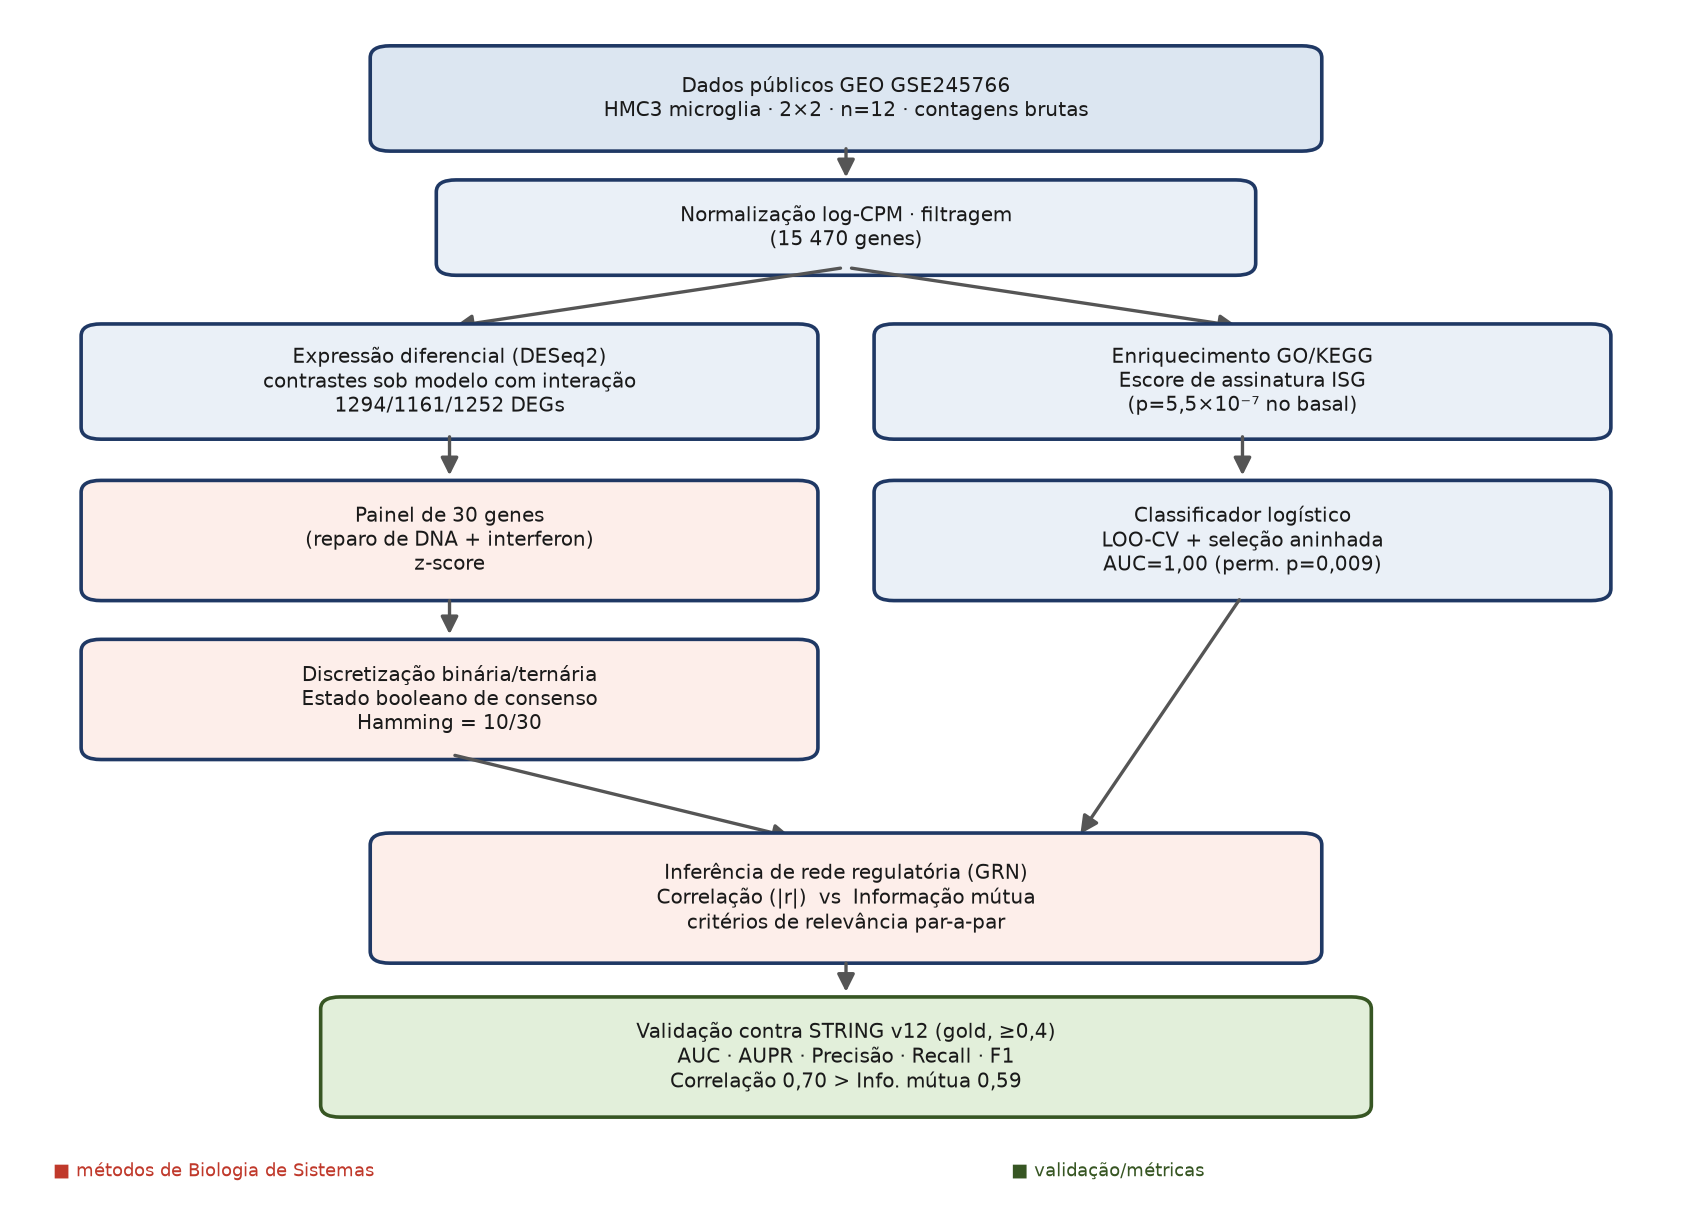
\includegraphics[width=0.92\textwidth]{figure_fluxograma.png}
\caption{Fluxograma do \emph{pipeline} analítico. Os blocos em tom avermelhado
destacam os métodos de: discretização, modelagem booleana e
inferência de rede; o bloco verde indica a etapa de validação por métricas
contra a rede de referência STRING.}
\label{fig:fluxo}
\end{figure}

Os dados de expressão gênica foram obtidos do conjunto público
GSE245766~\cite{Madsen2023}, composto por experimentos de RNA-seq realizados em
células de microglia humana da linhagem HMC3. O delineamento experimental seguiu
um modelo fatorial \(2\times2\), considerando os fatores genótipo
(\gene{APTX} \emph{knockout} [APTX-KO] versus tipo selvagem [WT]) e estímulo
imune (estimulado [IS] versus não estimulado [NS]), totalizando 12 amostras
(3 réplicas biológicas por condição).

As contagens gênicas foram submetidas a controle de qualidade e filtragem de
genes com baixa expressão utilizando a função \texttt{filterByExpr} do pacote
\textsf{edgeR}, resultando na retenção de \num{15600} genes para as análises
subsequentes. Em seguida, os dados foram transformados por estabilização de
variância utilizando a função \texttt{vst} do pacote \textsf{DESeq2}.

A análise de expressão diferencial foi conduzida com o pacote \textsf{DESeq2},
utilizando o modelo estatístico
\(\sim \text{gen\'otipo} + \text{est\'imulo} + \text{gen\'otipo}\!:\!\text{est\'imulo}\).
Foram considerados diferencialmente expressos os genes com valor ajustado de
\(p\) (\(p_{\mathrm{adj}}\)) inferior a \num{0.05} e magnitude absoluta de
alteração de expressão superior a \(|\logfc{}| > 1\).

As análises de co-expressão gênica foram realizadas por meio do método
\emph{Weighted Gene Co-expression Network Analysis} (WGCNA), utilizando redes do
tipo \emph{signed}. Considerando o número reduzido de amostras, a construção da
rede teve caráter exploratório. Como não foi observado ajuste satisfatório ao
critério de topologia livre de escala (\emph{scale-free topology}), adotou-se o
parâmetro \(\beta = 18\), conforme recomendação do próprio \emph{framework} para
redes \emph{signed}. Alterações na arquitetura das redes de co-expressão entre
os grupos APTX-KO e WT foram investigadas utilizando o método CoDiNA
(\emph{Co-expression Differential Network Analysis}).

A interpretação funcional dos DEGs foi realizada por análise de enriquecimento
utilizando o pacote \textsf{clusterProfiler}, considerando termos do
Gene Ontology (GO -- \emph{Biological Process}) e vias da base KEGG, com
correção para múltiplos testes. Para avaliar a capacidade discriminativa entre
os grupos KO e WT, foi empregado um modelo \emph{Elastic Net}
(\textsf{glmnet}) com validação cruzada \emph{leave-one-out} (LOO-CV). A fim de
minimizar viés de seleção de atributos, a identificação de DEGs foi repetida
independentemente dentro de cada iteração da validação cruzada, conforme
recomendado por Ambroise e McLachlan~\cite{Ambroise2002}. Por fim, a análise de
Medicina de Redes foi conduzida utilizando a base STRINGdb v12.0 para
\emph{Homo sapiens} (score \(\geq 400\)), com propriedades topológicas
(grau, intermediação, proximidade) calculadas pelo pacote \textsf{igraph}.

\paragraph{Reanálise independente.} Para verificar a reprodutibilidade e a
robustez dos achados, as contagens brutas públicas foram reprocessadas de forma
independente (GLM binomial negativo equivalente ao DESeq2; mapeamento
Ensembl\(\rightarrow\)símbolo via mygene.info; enriquecimento via Enrichr
GO/KEGG; classificador logístico com seleção de atributos aninhada e teste de
permutação de rótulos). Essa etapa reteve \num{15470} genes após filtragem,
praticamente idêntico ao pipeline original.

\paragraph{Discretização e modelagem booleana.} Para aplicar os métodos, definiu-se um painel de 30 genes composto pelo módulo das
ataxias de reparo de DNA (\gene{APTX}, \gene{TDP1}, \gene{XRCC1}, \gene{XRCC4},
\gene{LIG3}, \gene{LIG4}, \gene{PNKP}, \gene{SETX}, \gene{PARP1}, \gene{ATM}) e
por um conjunto de genes da imunidade inata/interferon (\gene{IFI44L},
\gene{OAS1}--\gene{OAS3}, \gene{ISG15}, \gene{MX1}/\gene{MX2}, \gene{RSAD2},
\gene{IFIT1}/\gene{IFIT3}, \gene{STAT1}/\gene{STAT2}, \gene{IRF7},
\gene{DDX58}/RIG-I, entre outros). Os perfis de \emph{log}-CPM foram
padronizados por gene (transformação \emph{z-score}) e, em seguida,
\emph{quantizados} em duas representações discretas: (i) \emph{quantização binária}, atribuindo \(1\) (superexpresso)
quando \(z>0\) e \(0\) (subexpresso) caso contrário; e (ii) \emph{quantização
ternária}, atribuindo \(+1\), \(0\) ou \(-1\) segundo bandas de
\(\pm 0{,}5\) desvio-padrão. A partir da representação binária, definiu-se, por
votação majoritária entre as réplicas, um \emph{estado booleano de consenso}
para cada genótipo (WT e KO); a diferença entre os dois estados foi quantificada
pela \emph{distância de Hamming}, número de genes que alternam entre os estados
ON/OFF.

\paragraph{Inferência de rede regulatória e validação.} A rede de co-regulação
do painel foi inferida por dois critérios de relevância:
\emph{correlação de Pearson} (dependência linear par-a-par, \(|r|\)) e
\emph{informação mútua} (dependência estatística geral, estimador de vizinhos
mais próximos do \textsf{scikit-learn}). Cada par de genes recebeu, assim, um
escore de associação. As redes inferidas foram validadas contra uma rede de
referência (\emph{gold standard}) construída a partir da base STRING v12.0
(interações com \emph{score} \(\geq 0{,}4\) entre os genes do painel; 212
arestas de referência dentre 435 pares possíveis). O desempenho foi avaliado com
a matriz de confusão e as métricas correspondentes - precisão, \emph{recall}
(sensibilidade), \emph{F1}, área sob a curva ROC (AUC) e área sob a curva
precisão-\emph{recall} (AUPR) - , comparando os dois métodos entre si e contra
um classificador aleatório (AUPR igual à prevalência de arestas). Para as
métricas pontuais, adotou-se como limiar a seleção das \(k\) arestas de maior
escore, com \(k\) igual ao número de arestas de referência.

% ======================================================================
\section*{Resultados}

\subsection*{Expressão diferencial (DESeq2)}

Foram identificados \num{1221} DEGs entre as condições APTX-KO e WT
(Tabela~\ref{tab:deg}). Os genes mais significativamente alterados incluem
\gene{IFI44L}, \gene{IFITM1}, \gene{OAS1}, \gene{IFI6}, \gene{IFIT1},
\gene{USP18}, \gene{BST2} e \gene{DDX58} (RIG-I) (Tabela~\ref{tab:topdeg}).
Muitos desses genes estão descritos na literatura como participantes de
respostas mediadas por interferon e mecanismos de defesa antiviral, sugerindo
uma modulação de processos relacionados à imunidade inata, hipótese
posteriormente explorada pelas análises de enriquecimento funcional.

\begin{table}[htbp]
\centering
\caption{Número de genes diferencialmente expressos por contraste
(\(p_{\mathrm{adj}} < 0{,}05\) e \(|\logfc{}| > 1\)).}
\label{tab:deg}
\begin{tabular}{lrrr}
\toprule
\textbf{Contraste} & \textbf{DEGs} & \textbf{Up} & \textbf{Down} \\
\midrule
Genótipo (KO vs WT)            & \num{1221} & 554 & 667 \\
Estímulo (IS vs NS)            & \num{1291} & 936 & 355 \\
Interação genótipo \(\times\) estímulo & 209 & 82 & 127 \\
\bottomrule
\end{tabular}
\end{table}

\begin{table}[htbp]
\centering
\caption{Top 12 DEGs do efeito do genótipo (KO vs WT). Predomina o programa
interferon/antiviral. \(p_{\mathrm{adj}}\) abaixo do limite de precisão numérica
indicado como \(< 2{,}2\times10^{-16}\).}
\label{tab:topdeg}
\begin{tabular}{lrl}
\toprule
\textbf{Gene} & \textbf{\logfc{}} & \textbf{\(p_{\mathrm{adj}}\)} \\
\midrule
\gene{IFI44L} & \(-4{,}84\) & \(< 2{,}2\times10^{-16}\) \\
\gene{IFITM1} & \(-3{,}42\) & \(< 2{,}2\times10^{-16}\) \\
\gene{GOLGA4} & \(+3{,}29\) & \(< 2{,}2\times10^{-16}\) \\
\gene{BST2}   & \(-3{,}25\) & \(< 2{,}2\times10^{-16}\) \\
\gene{CDH13}  & \(+3{,}08\) & \(< 2{,}2\times10^{-16}\) \\
\gene{OAS1}   & \(-2{,}78\) & \(< 2{,}2\times10^{-16}\) \\
\gene{RIGI}   & \(-2{,}42\) & \(< 2{,}2\times10^{-16}\) \\
\gene{IFI44}  & \(-2{,}40\) & \(< 2{,}2\times10^{-16}\) \\
\gene{PSG1}   & \(+2{,}36\) & \(< 2{,}2\times10^{-16}\) \\
\gene{USP18}  & \(-2{,}31\) & \(< 2{,}2\times10^{-16}\) \\
\gene{IFI6}   & \(-2{,}30\) & \(< 2{,}2\times10^{-16}\) \\
\gene{IFIT1}  & \(-2{,}17\) & \(< 2{,}2\times10^{-16}\) \\
\bottomrule
\end{tabular}
\end{table}

\paragraph{O ``efeito do genótipo'' depende do contraste.} No modelo com
interação, o coeficiente principal de genótipo testa KO vs WT \emph{apenas no
nível de referência do estímulo} (células não estimuladas, NS). A reanálise
extraiu os três contrastes possíveis (Fig~\ref{fig:reanalise}a): KO-vs-WT em
NS (\num{1294} DEGs, reproduzindo o número original), KO-vs-WT em IS
(\num{1161} DEGs) e o efeito marginal de genótipo (modelo aditivo; \num{1252}
DEGs). A sobreposição entre as listas em NS e IS é de apenas
\(\text{Jaccard} = 0{,}50\) (822 DEGs em comum; 472 exclusivos de NS; 339
exclusivos de IS), indicando que quase metade dos DEGs de genótipo muda conforme
o contraste. Portanto, descreve-se o contraste principal como
``KO vs WT em células não estimuladas''.

\subsection*{Co-expressão (WGCNA e CoDiNA)}

Com \(n=12\) o ajuste \emph{scale-free} é fraco; adotou-se \(\beta=18\). A
análise WGCNA identificou oito módulos de co-expressão
(Tabela~\ref{tab:wgcna}). Os módulos \emph{yellow} (\(r=-0{,}98\)) e \emph{blue}
(\(r=0{,}96\)) apresentaram as correlações mais elevadas com o fator genótipo,
enquanto \emph{turquoise} (\(r=0{,}98\)) e \emph{red} (\(r=-0{,}96\))
predominaram no fator estímulo. Entre os genes previamente selecionados, apenas
\gene{SETX} foi alocado ao módulo \emph{turquoise}, enquanto \gene{TDP1} e
\gene{LIG3} foram alocados ao módulo \emph{blue}; \gene{APTX} não foi incluído na
rede construída a partir dos \num{5000} genes mais variáveis, o que pode refletir
sua limitada variação transcricional nas condições avaliadas.

A comparação das redes por CoDiNA identificou \num{1454} nós conservados entre as
condições, além de 224 nós com conectividade específica do grupo APTX-KO e 291
nós com conectividade específica do grupo WT, sugerindo alterações nos padrões de
conectividade associados à perda de \gene{APTX}.

\begin{table}[htbp]
\centering
\caption{Correlação entre \emph{eigengenes} dos módulos e os fatores
experimentais. Com \(n=12\), os \(p\)-valores são nominais/otimistas e a
interpretação deve ser feita em nível de módulo.}
\label{tab:wgcna}
\begin{tabular}{lrrrr}
\toprule
\textbf{Módulo} & \textbf{\(r_{\text{gen}}\)} & \textbf{\(p_{\text{gen}}\)}
& \textbf{\(r_{\text{est}}\)} & \textbf{\(p_{\text{est}}\)} \\
\midrule
yellow    & \(-0{,}98\) & \(1{,}3\times10^{-8}\) & \(-0{,}17\) & \(5{,}9\times10^{-1}\) \\
blue      & \(+0{,}96\) & \(9{,}3\times10^{-7}\) & \(+0{,}28\) & \(3{,}8\times10^{-1}\) \\
green     & \(+0{,}89\) & \(8{,}7\times10^{-5}\) & \(-0{,}44\) & \(1{,}5\times10^{-1}\) \\
brown     & \(-0{,}83\) & \(8{,}5\times10^{-4}\) & \(+0{,}54\) & \(7{,}2\times10^{-2}\) \\
black     & \(-0{,}60\) & \(3{,}9\times10^{-2}\) & \(-0{,}76\) & \(3{,}9\times10^{-3}\) \\
red       & \(+0{,}23\) & \(4{,}7\times10^{-1}\) & \(-0{,}96\) & \(1{,}2\times10^{-6}\) \\
turquoise & \(-0{,}06\) & \(8{,}6\times10^{-1}\) & \(+0{,}98\) & \(1{,}1\times10^{-8}\) \\
grey      & \(-0{,}05\) & \(8{,}7\times10^{-1}\) & \(-0{,}08\) & \(8{,}1\times10^{-1}\) \\
\bottomrule
\end{tabular}
\end{table}

\subsection*{Enriquecimento funcional (GO/KEGG)}

As análises de enriquecimento evidenciaram predominância de processos
relacionados à resposta antiviral e à imunidade inata. Entre os termos GO
(\emph{Biological Process}) mais significativos destacam-se
\emph{type I interferon signaling}, \emph{cellular response to type I
interferon}, \emph{negative regulation of viral genome replication},
\emph{defense response to virus} e \emph{cytokine-mediated signaling}
(todos \(p_{\mathrm{adj}} < 10^{-6}\)). Entre as vias KEGG canônicas
destacam-se \emph{Cytokine-cytokine receptor interaction}, \emph{NF-kappa B
signaling pathway}, \emph{NOD-like receptor signaling pathway} e
\emph{Influenza A}. A reanálise confirmou essa biologia e evidenciou que a
escolha do universo de referência (genoma inteiro versus genes expressos)
altera materialmente o número de termos significativos (GO BP: 130 versus 231;
KEGG: 20 versus 36), reforçando a importância de declarar explicitamente o
universo de \emph{background}.

\subsection*{Assinatura de interferon}

Para quantificar o programa antiviral, calculou-se um escore de assinatura de
genes estimulados por interferon (ISGs) por amostra (Fig~\ref{fig:reanalise}b).
O programa está fortemente reprimido no KO \emph{especificamente no basal}
(NS: WT \(-0{,}26\) vs KO \(-1{,}36\); \(p = 5{,}5\times10^{-7}\)), enquanto sob
estímulo os grupos quase convergem (IS: WT \(+0{,}89\) vs KO \(+0{,}74\);
\(p = 5{,}1\times10^{-3}\)). Esse padrão, redução do tônus basal de
sinalização de interferon, é exatamente o esperado se as vias cGAS-STING e
RIG-I-MAVS estiverem menos ativas na ausência de \gene{APTX}, e explica por que
o teste marginal de genótipo é comparativamente fraco: o efeito é dirigido pela
interação (basal), não uniforme entre estímulos.

\subsection*{Classificação (LOO-CV) e teste de permutação}

Ambos os modelos (DEGs com seleção aninhada; \emph{eigengenes} do WGCNA)
alcançaram desempenho máximo (AUC \(=1{,}00\); 12/12 amostras corretamente
classificadas). Para avaliar se esse resultado é significativo dado o tamanho
amostral, realizou-se um teste de permutação de rótulos (\num{1000} permutações,
com todo o pipeline (incluindo a seleção aninhada) refeito em cada
permutação; Fig~\ref{fig:reanalise}c). A distribuição nula centrou-se em
AUC \(=0{,}34\) (95\({}^{\text{o}}\) percentil \(=0{,}78\)), com \(p\) empírico
\(= 0{,}009\). Assim, AUC \(=1{,}00\) é estatisticamente significativo e não um
artefato do \(n\) pequeno. Ressalva-se, contudo, que o modelo baseado em
\emph{eigengenes} do WGCNA permanece sujeito a vazamento de informação, pois os
módulos foram derivados usando as 12 amostras simultaneamente; sua interpretação
deve ser cautelosa.

\begin{figure}[htbp]
\centering
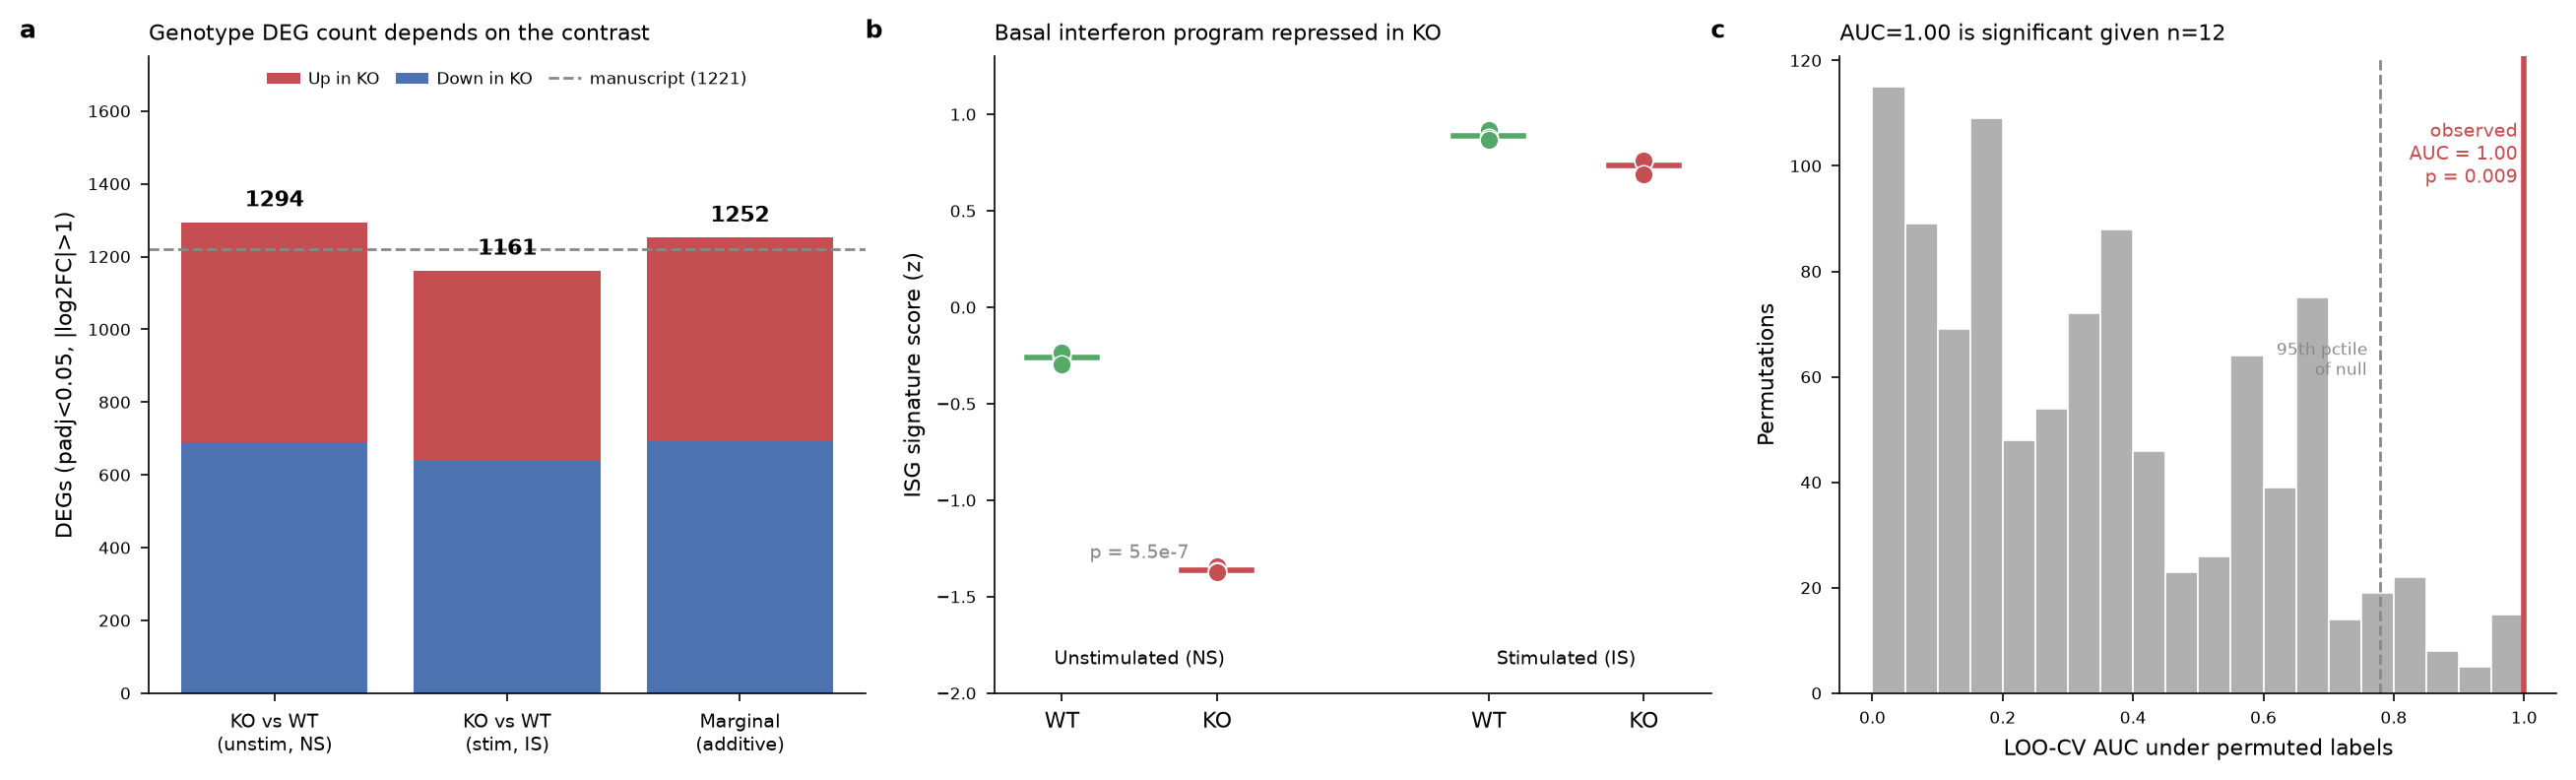
\includegraphics[width=\textwidth]{figure_reanalysis.png}
\caption{Reanálise independente das contagens brutas do GSE245766.
\textbf{(a)} O número de DEGs do efeito do genótipo depende do contraste
extraído sob o modelo com interação; a linha tracejada indica o valor original
(\num{1221}). \textbf{(b)} Escore de assinatura de ISG por grupo: o programa de
interferon está reprimido no KO especificamente no basal (NS). \textbf{(c)}
Distribuição nula do AUC de LOO-CV sob permutação de rótulos; o valor observado
(\num{1.00}) é significativo (\(p=0{,}009\)).}
\label{fig:reanalise}
\end{figure}

\subsection*{Discretização e estados booleanos}

A quantização ternária dos 30 genes do painel evidenciou um padrão dominado pelo
estímulo imune no bloco de genes de interferon, coerente com os resultados de
expressão diferencial, e alterações mais discretas no bloco de reparo de DNA
(Fig~\ref{fig:disc}a). A partir da representação binária, os estados booleanos
de consenso dos genótipos WT e KO diferem em uma \emph{distância de Hamming} de
\num{10}/\num{30} genes (Fig~\ref{fig:disc}b): alternam de estado \gene{TDP1},
\gene{XRCC4}, \gene{LIG3}, \gene{PNKP} e \gene{ATM} (bloco de reparo) e
\gene{IFI44L}, \gene{IFI44}, \gene{IFI6}, \gene{BST2} e \gene{IRF7} (bloco imune).
Essa análise discreta recupera, de forma simplificada e interpretável, a
coexistência de alterações no módulo de reparo e no programa de interferon já
observada pelas análises contínuas.

\begin{figure}[htbp]
\centering
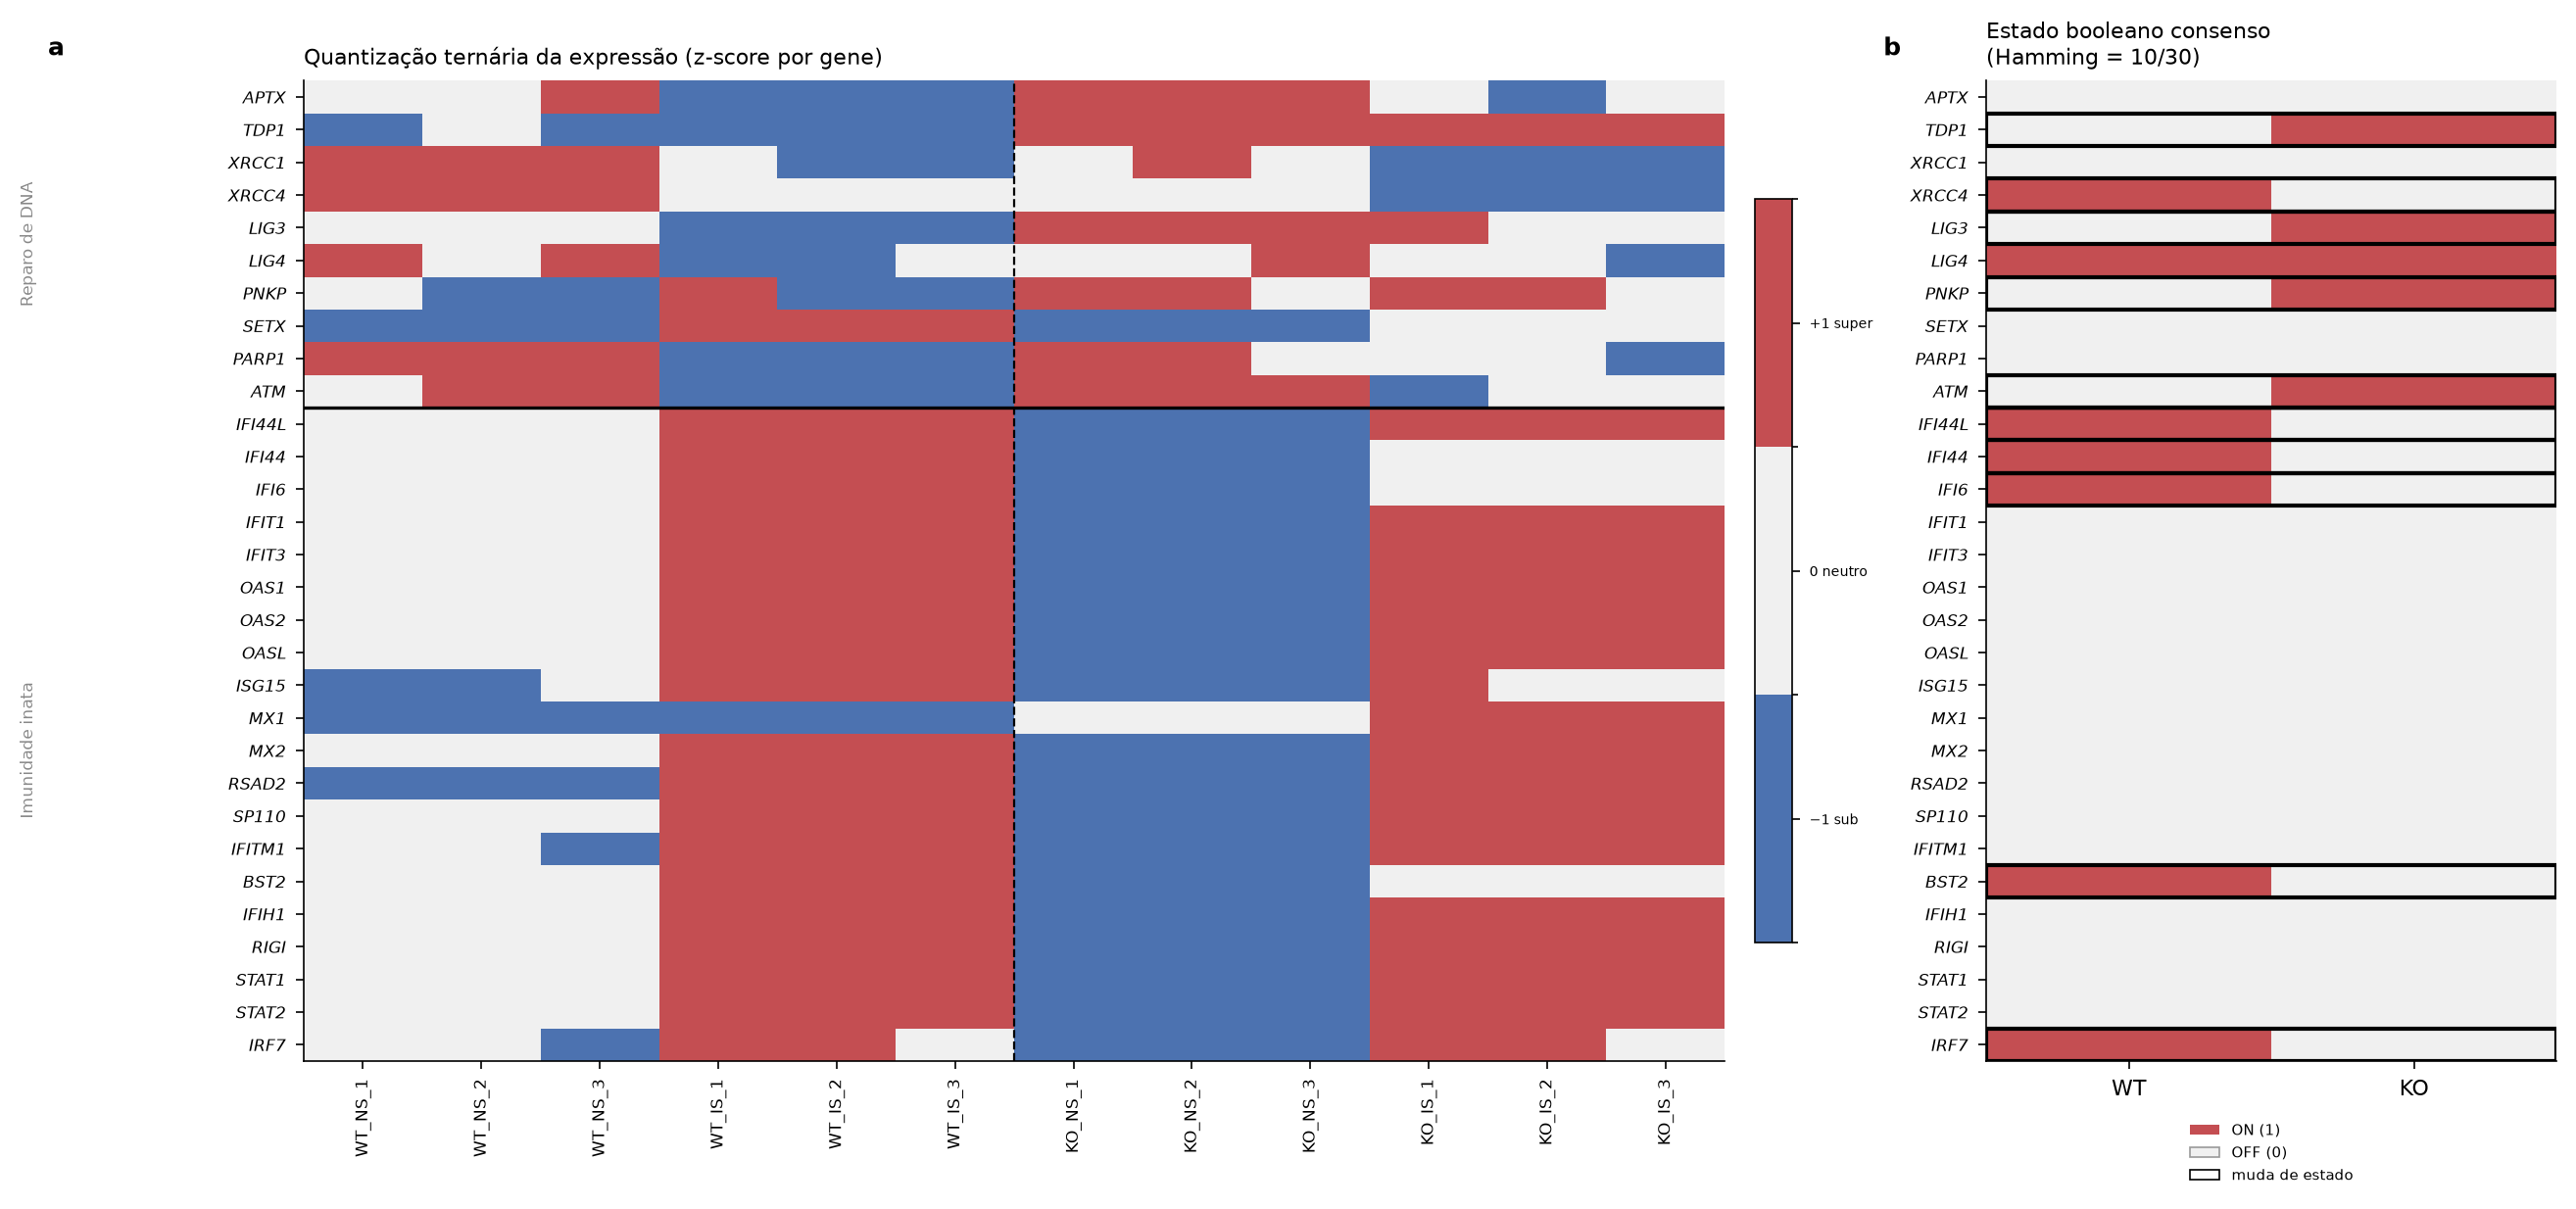
\includegraphics[width=\textwidth]{figure_discretizacao.png}
\caption{Discretização e modelagem booleana do painel de 30 genes.
\textbf{(a)} Quantização ternária (\emph{z-score} por gene): \(+1\) superexpresso
(vermelho), \(0\) neutro (cinza), \(-1\) subexpresso (azul). A linha horizontal
separa o módulo de reparo de DNA (topo) do módulo de imunidade inata; a linha
vertical tracejada separa amostras não estimuladas (NS) de estimuladas (IS).
\textbf{(b)} Estado booleano de consenso por genótipo (votação majoritária das
réplicas); genes destacados alternam de estado entre WT e KO
(distância de Hamming \(= 10/30\)).}
\label{fig:disc}
\end{figure}

\subsection*{Inferência de rede regulatória: correlação vs.\ informação mútua}

A rede de co-regulação do painel foi inferida
por dois critérios, correlação de Pearson e informação mútua, e validada
contra a rede de referência STRING (Fig~\ref{fig:grn}; Tabela~\ref{tab:grn}).
A correlação apresentou desempenho superior em todas as métricas
(AUC \(=0{,}70\); AUPR \(=0{,}71\); F1 \(=0{,}63\)) em comparação à informação
mútua (AUC \(=0{,}59\); AUPR \(=0{,}55\); F1 \(=0{,}59\)), ambas acima do
classificador aleatório (AUPR \(=0{,}49\)). Esse resultado é coerente com as
propriedades dos métodos discutidas em aula: estimadores de informação mútua
requerem mais amostras para estabilizar, ao passo que a correlação linear é
robusta em regimes de \(M \ll N\) (aqui, apenas \(M=12\) amostras), embora seja
incapaz de capturar dependências não lineares ou relações \(N\!:\!1\).
Metodologicamente, isso ilustra o compromisso entre a generalidade do critério de
relevância e a estabilidade estatística sob amostragem limitada.

\begin{table}[htbp]
\centering
\caption{Validação das redes inferidas contra o \emph{gold standard} STRING
(\(\geq 0{,}4\); 212 arestas dentre 435 pares). Métricas pontuais no limiar
top-\(k\) (\(k=212\)). Melhor valor por métrica em negrito.}
\label{tab:grn}
\begin{tabular}{lccccc}
\toprule
\textbf{Método} & \textbf{AUC} & \textbf{AUPR} & \textbf{Precisão} & \textbf{Recall} & \textbf{F1} \\
\midrule
Correlação (\(|r|\)) & \textbf{0{,}70} & \textbf{0{,}71} & \textbf{0{,}63} & \textbf{0{,}63} & \textbf{0{,}63} \\
Informação mútua     & 0{,}59 & 0{,}55 & 0{,}59 & 0{,}59 & 0{,}59 \\
\midrule
Aleatório (prevalência) & 0{,}50 & 0{,}49 & --- & --- & --- \\
\bottomrule
\end{tabular}
\end{table}

\begin{figure}[htbp]
\centering
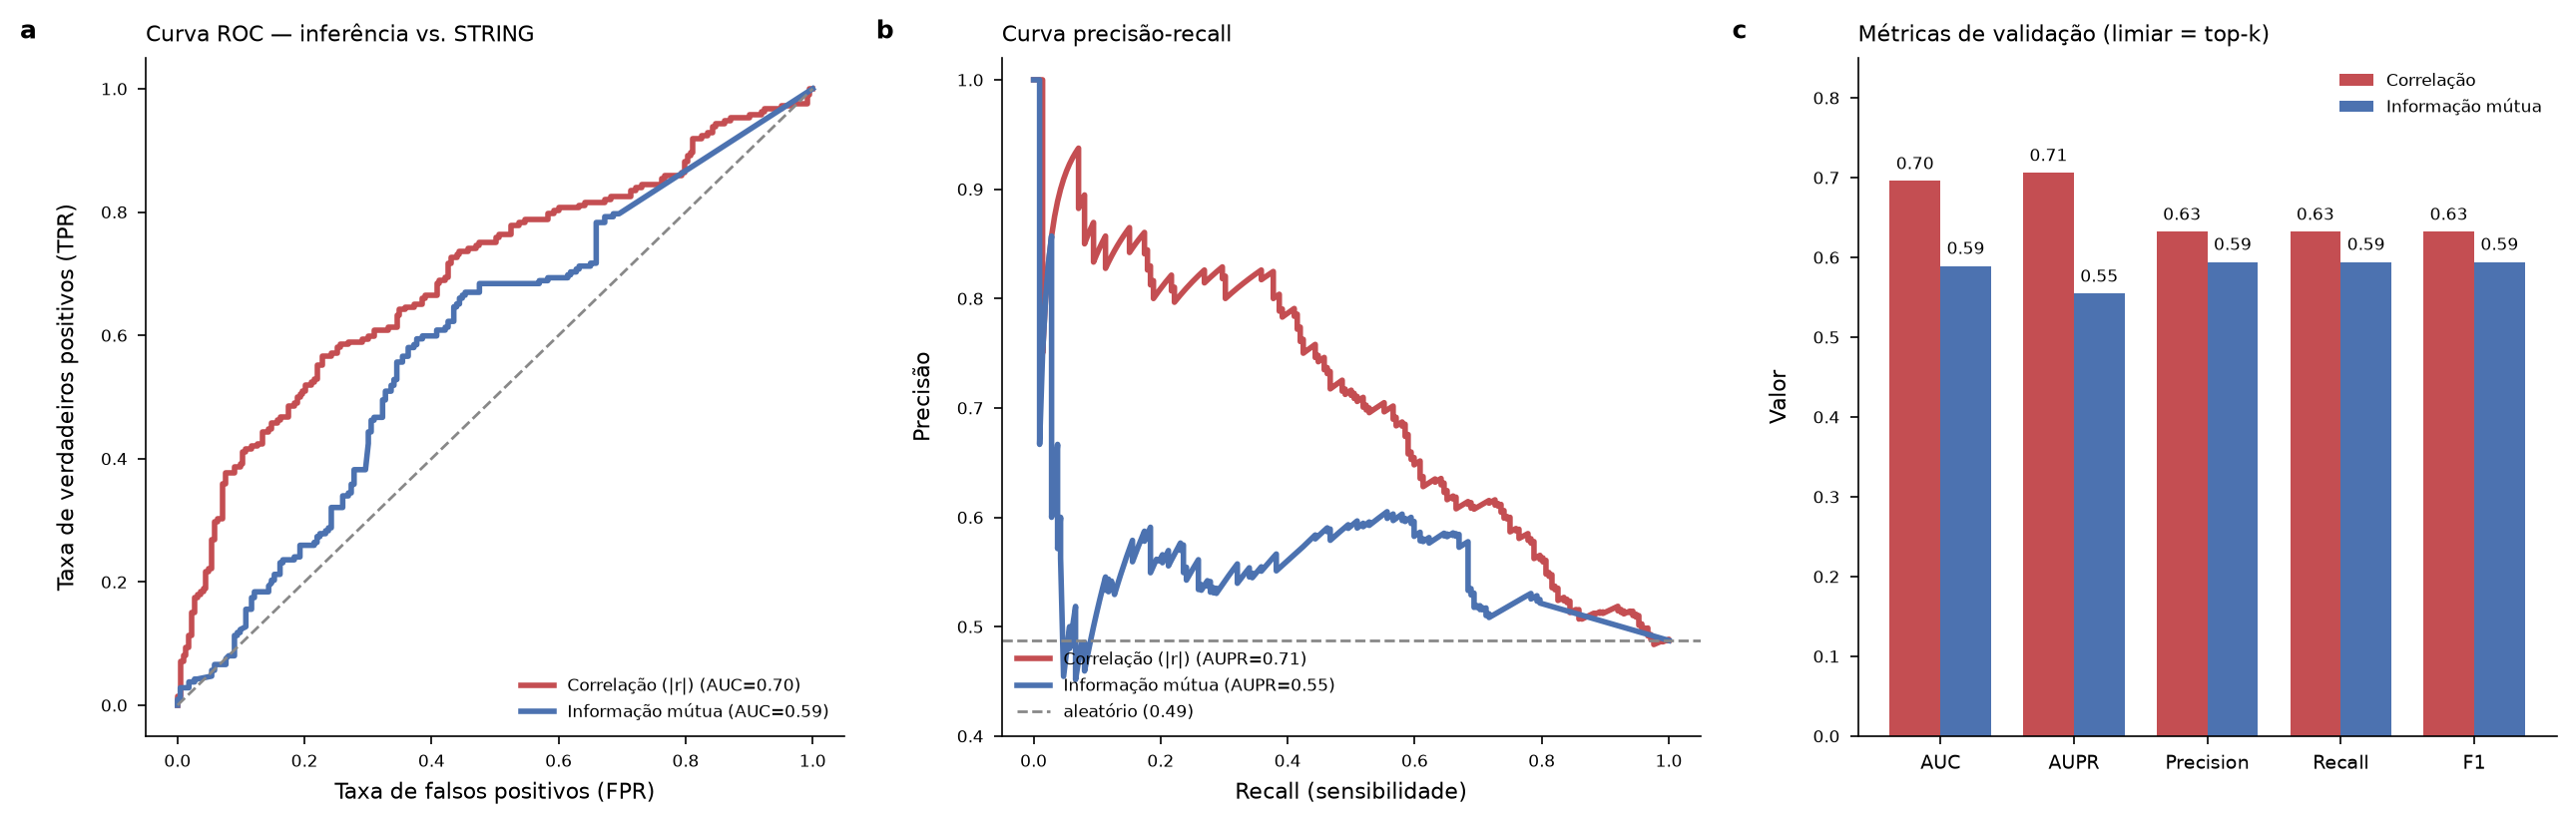
\includegraphics[width=\textwidth]{figure_grn_inference.png}
\caption{Inferência da rede de co-regulação do painel validada contra STRING.
\textbf{(a)} Curvas ROC e \textbf{(b)} curvas precisão-\emph{recall} para os dois
critérios de relevância; a linha tracejada indica o classificador aleatório.
\textbf{(c)} Métricas de validação no limiar top-\(k\). A correlação supera a
informação mútua em todas as métricas neste regime de poucas amostras
(\(M=12\)).}
\label{fig:grn}
\end{figure}

\subsection*{Medicina de Redes (STRINGdb)}

A rede de interações dos dez genes-semente (Figura~\ref{fig:netmed}) mostrou-se
significativamente mais conectada que o esperado ao acaso (\num{41} interações
observadas \emph{vs.}\ \num{2} esperadas; \(p < 10^{-16}\)), confirmando que
formam um módulo funcional coeso de reparo de DNA. \gene{ATM} e \gene{PARP1}
apresentaram os maiores valores de grau e intermediação, destacando-se como os
nós mais conectados do módulo (Tabela~\ref{tab:string}). O \gene{APTX}, embora com grau relativamente menor,
exibiu elevada centralidade de intermediação (\(\sim\!\num{12430}\)), sugerindo
função de conexão entre subconjuntos da rede, padrão compatível com seu papel
no reparo de quebras de fita simples (SSBR). Embora nenhum gene-semente tenha
ultrapassado \(|\logfc{}| > 1\), cinco genes (\gene{APTX}, \gene{TDP1},
\gene{XRCC1}, \gene{XRCC4} e \gene{LIG3}) apresentaram significância estatística
após correção, sugerindo alterações discretas em componentes do módulo de
reparo.

\begin{table}[htbp]
\centering
\caption{Centralidade dos genes-semente na rede STRING e significância no KO
(\(p_{\mathrm{adj}} < 0{,}05\)).}
\label{tab:string}
\begin{tabular}{lrrc}
\toprule
\textbf{Gene} & \textbf{Grau} & \textbf{Intermediação} & \textbf{Signif.\ KO} \\
\midrule
\gene{ATM}   & 770 & \num{55681} & não \\
\gene{PARP1} & 710 & \num{53233} & não \\
\gene{XRCC1} & 229 & \num{5603}  & sim \\
\gene{LIG3}  & 206 & \num{2916}  & sim \\
\gene{LIG4}  & 200 & \num{5541}  & não \\
\gene{SETX}  & 168 & \num{11825} & não \\
\gene{XRCC4} & 139 & \num{3104}  & sim \\
\gene{APTX}  & 113 & \num{12430} & sim \\
\gene{PNKP}  & 107 & \num{7003}  & não \\
\gene{TDP1}  &  88 & \num{2061}  & sim \\
\bottomrule
\end{tabular}
\end{table}

\begin{figure}[htbp]
\centering
\includegraphics[width=0.6\textwidth]{results/figures/netmed_seed_module_trim.png}
\caption{{\bf Módulo de reparo de DNA dos genes-semente na rede STRING.}
Rede de interações proteína--proteína (STRINGdb, \emph{Homo sapiens}, versão
12.0) dos dez genes-semente das ataxias de reparo. O conjunto exibe
enriquecimento significativo de interações (\num{41} observadas \emph{vs.}\
\num{2} esperadas ao acaso; \(p < 10^{-16}\)), evidenciando um módulo funcional
coeso. O \gene{APTX} integra-se ao módulo com elevada centralidade de
intermediação (Tabela~\ref{tab:string}), compatível com seu papel de conexão no
reparo de quebras de fita simples.}
\label{fig:netmed}
\end{figure}

% ======================================================================
\section*{Discussão}

Os resultados sugerem que a perda de \gene{APTX} está associada a alterações mais
pronunciadas em programas relacionados à imunidade inata do que na expressão dos
genes clássicos de reparo de DNA. Os genes diretamente envolvidos no reparo
apresentaram alterações transcricionais discretas, compatível com a função
predominantemente enzimática atribuída à aprataxina.

Um achado que merece destaque é que o mRNA de \gene{APTX} \emph{não está reduzido}
no \emph{knockout}, a reanálise confirmou \logfc{} \(=+0{,}21\)
(\(p_{\mathrm{adj}}\) significativo), reproduzindo o \(+0{,}27\) original. Isso
indica que o modelo é um \emph{knockout funcional} (lesão gerando transcrito
estável, porém proteína não-funcional), e não um \emph{knockout} de expressão.
Portanto, o achado fica descrito como ``perda de função de \gene{APTX}''.

Em contraste, foram observadas alterações expressivas em genes e vias associadas
à resposta antiviral e à sinalização por interferon, incluindo \gene{DDX58}
(RIG-I), \gene{OAS1} e diversos ISGs. Essa tendência foi consistente nas análises
de expressão diferencial, enriquecimento funcional, co-expressão diferencial e no
escore de assinatura de ISG, apontando para processos de resposta a vírus,
sinalização por interferon tipo I e II, NF-\(\kappa\)B e receptores NOD-like.
Esses achados são compatíveis com evidências recentes de uma interface funcional
entre os mecanismos de reparo de DNA mediados por \gene{APTX} e as vias da
imunidade inata (eixos cGAS-STING e RIG-I-MAVS)~\cite{Madsen2023}. Importante:
a direção observada é concordante com o estudo de
origem, o que confere à presente reanálise o caráter de \emph{validação
independente}.

Na análise de redes de interação proteína-proteína, o \gene{APTX} apresentou
elevada centralidade de intermediação, sugerindo potencial participação na
conexão entre componentes do módulo das ataxias de reparo de DNA, enquanto
\gene{ATM} e \gene{PARP1} destacaram-se como os nós mais centrais.

A aplicação dos métodos de discretização, modelagem
booleana e inferência de rede regulatória, agregou uma perspectiva
complementar às análises contínuas. A representação booleana de consenso resumiu
as alterações de estado entre WT e KO (distância de Hamming \(=10/30\)),
localizando-as simultaneamente nos blocos de reparo de DNA e de interferon. Na
inferência da rede de co-regulação, a comparação entre correlação e informação
mútua contra a rede de referência STRING evidenciou a superioridade da
correlação neste regime de poucas amostras. Esse achado ilustra uma propriedade
metodológica central: critérios de relevância mais gerais, como a informação
mútua, capturam dependências não lineares e relações multivariadas, mas exigem
maior número de amostras para uma estimativa estável; sob \(M \ll N\), a
correlação linear, apesar de suas limitações, tende a produzir inferências mais
robustas. Trata-se de uma limitação devido ao tamanho da amostra (\(n=12\)), e não ao modelo de informação mútua em si.

\subsection*{Limitações}

\begin{enumerate}
\item O estudo foi realizado em linhagem celular de microglia humana (HMC3), e
não em amostras de pacientes com AOA1; os resultados devem ser interpretados no
contexto de um modelo \emph{in vitro}. O reduzido número de amostras
(\(n=3\) por condição) confere caráter exploratório às análises de co-expressão.
\item O critério de ajuste à topologia livre de escala não foi plenamente
atendido; \(\beta=18\) foi definido por recomendação do \emph{framework} WGCNA
para redes \emph{signed}, e não estimado diretamente dos dados.
\item Os modelos de classificação apresentaram AUC \(=1{,}00\); embora o teste de
permutação confirme a significância, o reduzido tamanho amostral limita a
avaliação da capacidade de generalização, e a forte separação entre condições
torna a tarefa relativamente simples. Análises dos efeitos de estímulo ou
interação podem ser mais informativas.
\item Observou-se discreto aumento da expressão de \gene{APTX} no contraste KO
versus WT (\logfc{} \(=+0{,}27\)), possivelmente refletindo a estratégia de
geração do \emph{knockout} ou mecanismos compensatórios; a interpretação requer
confirmação das características moleculares do modelo original.
\end{enumerate}

% ======================================================================
\section*{Conclusão}

A perda de \gene{APTX} está associada predominantemente a alterações em programas
transcricionais relacionados à imunidade inata e à sinalização por interferon,
enquanto os genes clássicos de reparo de DNA apresentaram alterações mais
discretas. Entre os parceiros funcionais de \gene{APTX}, \gene{XRCC1},
\gene{XRCC4}, \gene{LIG3} e \gene{TDP1} apresentaram mudanças estatisticamente
significativas, embora de baixa magnitude. As análises de redes indicaram
elevada centralidade de intermediação para o \gene{APTX} dentro do módulo das
ataxias de reparo de DNA. Em conjunto, os achados são
consistentes com a hipótese de uma interface funcional entre mecanismos de reparo
de DNA e processos da imunidade inata no contexto da AOA1, fornecendo subsídios
para estudos funcionais futuros.

\paragraph{Principais contribuições.} O trabalho (i) reproduziu de forma
independente, a partir das contagens brutas, os resultados centrais do estudo
original; (ii) explicitou que o ``efeito do genótipo'' depende do contraste sob o
modelo com interação e que o \emph{knockout} é funcional, não de expressão; e
(iii) aplicou métodos de discretização, modelagem
booleana e inferência de rede regulatória, comparando dois critérios de
relevância contra uma rede de referência.

\paragraph{Dificuldades encontradas.} As principais dificuldades foram: o pequeno
tamanho amostral (\(n=12\)), que limita a estabilidade de estimadores como a
informação mútua e torna correlações otimistas; a dependência do resultado de
expressão diferencial em relação ao contraste extraído sob o modelo com
interação, exigindo cuidado na interpretação do ``efeito de genótipo''; a
anomalia aparente do \logfc{} de \gene{APTX} (positivo apesar do \emph{knockout}),
esclarecida como perda de função; a ausência do próprio \gene{APTX} em algumas
redes de co-expressão; e a escolha de limiares (discretização, \emph{score}
STRING, top-\(k\)) que influenciam as métricas e foram fixados de forma
justificada. A separação perfeita do classificador (AUC \(=1{,}00\)) exigiu um
teste de permutação para demonstrar significância apesar de \(n\) pequeno.

\paragraph{Síntese e justificativa.} Em síntese, a correlação superou a
informação mútua na inferência da rede (AUC \(0{,}70\) vs \(0{,}59\)), o que se
justifica pela maior robustez de estimadores lineares sob amostragem limitada, uma propriedade metodológica diretamente ligada ao desempenho observado. O
conjunto de análises converge para uma reprogramação a jusante do programa imune
inato como assinatura transcricional dominante da perda de \gene{APTX}.

% ======================================================================

\section*{Disponibilidade de código e dados}
Os dados de expressão são públicos (GEO, acesso GSE245766). O código completo de
reprocessamento (discretização, modelagem booleana, inferência de rede e
validação), os \emph{scripts} de geração de figuras e a fonte \LaTeX{} do artigo
estão disponíveis no repositório:
\begin{center}
\url{https://github.com/ppufpr/projeto-APTX-AOA1}
\end{center}

\section*{Declaração de uso de Inteligência Artificial}
\textbf{Ferramenta utilizada.} Assistente de IA generativa.\newline

\textbf{Como e onde foi utilizada.} A ferramenta foi empregada como apoio em
três etapas: (i) \emph{revisão crítica e compreensão} das referências bibliográficas e dos conceitos biológicos;
(ii) \emph{em scripts R e Python} na escrita e correção de bugs dos scripts; e
(iii) \emph{ajustes na formatação} em \LaTeX{}.\newline \newline
Todos os resultados numéricos foram
computados a partir dos dados reais (GSE245766), verificados por reexecução dos
\emph{scripts}.\newline

\textbf{Prompts utilizados (síntese).} As principais solicitações feitas à
ferramenta foram, em ordem cronológica:
\begin{enumerate}
\item ``Preciso de ajuda no entendimento de biologia do papers.''
\item ``Análise os bugs e realize a sugestão de correção do script...'' (correção e ajustes em problemas de compilação).
\item ``Ajude na correção da formatação do documento padrão \LaTeX{} com base no template fornecido.''
\end{enumerate}

% ======================================================================

\nolinenumbers

\begin{thebibliography}{10}

\bibitem{Madsen2023}
Madsen HB, Pease LI, Scanlan RL, Akbari M, Rasmussen LJ, Shanley DP, Bohr VA.
The DNA repair enzyme, aprataxin, plays a role in innate immune signaling.
\emph{Frontiers in Aging Neuroscience}. 2023;15:1290681.
doi:10.3389/fnagi.2023.1290681. (Dados: GEO GSE245766.)

\bibitem{Ambroise2002}
Ambroise C, McLachlan GJ.
Selection bias in gene extraction on the basis of microarray gene-expression
data. \emph{Proceedings of the National Academy of Sciences}.
2002;99(10):6562--6566. doi:10.1073/pnas.102102699.

\bibitem{Kauffman1969}
Kauffman SA.
Metabolic stability and epigenesis in randomly constructed genetic nets.
\emph{Journal of Theoretical Biology}. 1969;22(3):437--467.
doi:10.1016/0022-5193(69)90015-0.

\bibitem{Shmulevich2002}
Shmulevich I, Dougherty ER, Kim S, Zhang W.
Probabilistic Boolean networks: a rule-based uncertainty model for gene
regulatory networks. \emph{Bioinformatics}. 2002;18(2):261--274.
doi:10.1093/bioinformatics/18.2.261.

\bibitem{Butte2000}
Butte AJ, Kohane IS.
Mutual information relevance networks: functional genomic clustering using
pairwise entropy measurements. \emph{Pacific Symposium on Biocomputing}.
2000;5:418--429.

\bibitem{Szklarczyk2023}
Szklarczyk D, et al.
The STRING database in 2023: protein--protein association networks and
functional enrichment analyses. \emph{Nucleic Acids Research}.
2023;51(D1):D638--D646. doi:10.1093/nar/gkac1000.
\end{thebibliography}

\end{document}
